\documentclass[a4paper,11pt]{article}
\usepackage[verbose,a4paper,tmargin=2cm,bmargin=2.3cm,lmargin=2.5cm,rmargin=2.5cm]{geometry}
\usepackage[utf8]{inputenc}
\usepackage{polski}
\usepackage{amsmath}
\usepackage{amsfonts}
\usepackage{amssymb}
\usepackage{lastpage}
\usepackage{indentfirst}
\usepackage{verbatim}
\usepackage{graphicx}
\usepackage{hyperref}
\hypersetup{
    colorlinks = true,
    linkcolor = black,
    urlcolor = cyan
}
\usepackage{fancyhdr}
\usepackage{listings}
\usepackage{hyperref} 
\usepackage{booktabs}
\usepackage[table,xcdraw]{xcolor}
\usepackage{multirow}
\usepackage{tikz}
\usepackage{float}
\frenchspacing
\pagestyle{fancyplain}
\fancyhf{}



\usepackage{setspace}

\renewcommand{\headrulewidth}{0pt}
\renewcommand{\footrulewidth}{0.5pt}
\newcommand{\degree}{\ensuremath{^{\circ}}} 
% \fancyfoot[L]{Przetwarzanie i analiza dużych zbiorów danych: }
% \fancyfoot[R]{\thepage\ / \pageref{LastPage}}
\fancyfoot[L]{Przetwarzanie i analiza dużych zbiorów danych: \\Aleksandra Kowalczyk, Zbigniew Nowacki, Karol Podlewski}
\fancyfoot[R]{\phantom{a} \\ \thepage\ / \pageref{LastPage}}

\begin{document}

\begin{titlepage}
\begin{center}

\begin{tabular}{rcl}
\begin{tabular}{|r|}
\hline \\
\large{\underline{234073~~~~~~~~~~~~~~~~~~~~~~} }\\
\small{\textit{Numer indeksu}}\\
\large{\underline{Aleksandra Kowalczyk~~} }\\
\small{\textit{Imię i nazwisko}}\\\\ \hline
\end{tabular} 
&
\begin{tabular}{|r|}
\hline \\
\large{\underline{234102~~~~~~~~~~~~~~~~~~~~~~} }\\
\small{\textit{Numer indeksu}}\\
\large{\underline{Zbigniew Nowacki~~~~~~~} }\\
\small{\textit{Imię i nazwisko}}\\\\ \hline
\end{tabular} 
&
\begin{tabular}{|r|}
\hline \\
\large{\underline{234106~~~~~~~~~~~~~~~~~~~~~~} }\\
\small{\textit{Numer indeksu}}\\
\large{\underline{Karol Podlewski~~~~~~~~~~} }\\
\small{\textit{Imię i nazwisko}}\\\\ \hline
\end{tabular} 

\end{tabular}
~\\~\\~\\ 
\end{center}
\begin{tabular}{ll}
\LARGE{\textbf{Kierunek}}& \LARGE{Informatyka Stosowana} \\
\LARGE{\textbf{Stopień}}& \LARGE{II} \\
\LARGE{\textbf{Specjalizacja}}& \LARGE{Data Science} \\
\LARGE{\textbf{Semestr}}& \LARGE{2} \\\\
\LARGE{\textbf{Data oddania}}& \LARGE{18 listopada 2020} \\\\\\\\\\\\\\
\end{tabular}

\begin{center}
\textbf{\Huge{Przetwarzanie i analiza\\}}
\textbf{\Huge{dużych zbiorów danych\\~\\~\\~}}
\textbf{\Huge{Zadanie 3}}
\end{center}

\end{titlepage}

\setcounter{page}{2}

\setstretch{1.4}
\newpage
\section{Cel zadania}

Celem zadania była implementacja algorytmu \textit{k}-średnich z uwzględnieniem dwóch miar - euklidesowej oraz Manhattan - dla dwóch rozmieszeń centrów skupień - losowego oraz maksymalnie od siebie oddalonych centroidów według odległości euklidesowej. 

Dla każdej iteracji należało obliczyć funkcje kosztu $\phi(i)$ oraz $\psi(i)$, wygenerować wykresy oraz obliczyć procentową zmianę kosztu po 10 iteracjach algorytmu dla obydwu miar odległości z wskazaniem, które z dwóch początkowych rozmieszeń skupień pozwoliło uzyskać lepsze rezultaty.

Miara euklidesowa:
\begin{equation}
    \text{odległość:  } || a - b || = \sqrt{\sum_{i=1}^{d} (a_{i} - b_{i}) ^ 2 }
\end{equation}

\begin{equation}
    \text{koszt:  } \phi = \sum_{x \epsilon X} \min_{c \epsilon C} || x - c || ^ 2
\end{equation}

Miara Manhattan:
\begin{equation}
    \text{odległość:  } | a - b | = \sum_{i=1}^{d} | a_{i} - b_{i} |
\end{equation}

\begin{equation}
    \text{koszt:  } \psi =  \sum_{x \epsilon X} \min_{c \epsilon C} | x - c |
\end{equation}


\section{Opis implementacji}

Do implementacji zadania wykorzystano język Python wraz z API PySpark, które umożliwiło skorzystanie z możliwości języka Apache Spark w pythonowym kodzie. Wszystkie funkcje (odległości, kosztu) zostały zaimplementowane w programie, nie korzystano z bibliotek. 

\section{Uzyskane wyniki}

Analiza zajęła około 7 minut i 20 sekund.

\begin{table}[H]
\centering
\caption{Uzyskane wartości funkcji kosztu}
\label{tab:cost_results}
\begin{tabular}{@{}ccccc@{}}
\toprule
\multirow{2}{*}{Iteracja} & \multicolumn{2}{c}{Metryka euklidesowa} & \multicolumn{2}{c}{Metryka Manhattan} \\ \cmidrule(l){2-5} 
 & Plik 3b.txt & Plik 3c.txt & Plik 3b.txt & Plik 3c.txt \\ \midrule
1 & 623 660 345,30 & 438 747 790,02 & 550 117,14 & 1 433 739,31 \\
2 & 509 862 908,29 & 249 803 933,62 & 464 661,07 & 1 084 488,77 \\
3 & 485 480 681,87 & 194 494 814,40 & 471 200,04 & 973 431,71 \\
4 & 463 997 011,68 & 169 804 841,45 & 484 160,69 & 895 934,59 \\
5 & 460 969 266,57 & 156 295 748,80 & 489 251,72 & 865 128,33 \\
6 & 460 537 847,98 & 149 094 208,10 & 487 564,74 & 845 846,64 \\
7 & 460 313 099,65 & 142 508 531,61 & 483 404,05 & 827 219,58 \\
8 & 460 003 523,88 & 132 303 869,40 & 475 365,34 & 803 590,34 \\
9 & 459 570 539,31 & 117 170 969,83 & 474 924,05 & 756 039,51 \\
10 & 459 021 103,34 & 108 547 377,17 & 457 233,64 & 717 332,90 \\
11 & 458 490 656,19 & 102 237 203,31 & 447 495,09 & 694 587,92 \\
12 & 457 944 232,58 & 98 278 015,74 & 451 004,30 & 684 444,50 \\
13 & 457 558 005,19 & 95 630 226,12 & 451 222,09 & 674 574,74 \\
14 & 457 290 136,35 & 93 793 314,05 & 451 973,84 & 667 409,46 \\
15 & 457 050 555,05 & 92 377 131,96 & 451 585,35 & 663 556,62 \\
16 & 456 892 235,61 & 91 541 606,25 & 452 756,64 & 660 162,77 \\
17 & 456 703 630,73 & 91 045 573,83 & 452 893,79 & 656 041,32 \\
18 & 456 404 203,01 & 90 752 240,10 & 450 382,23 & 653 036,75 \\
19 & 456 177 800,54 & 90 470 170,18 & 450 023,96 & 651 112,42 \\
20 & 455 986 871,02 & 90 216 416,17 & 448 929,47 & 649 689,01 \\
\bottomrule
\end{tabular}
\end{table}

\small{
\[ \text{Zmiana względna } \phi_{3b.txt} \Big(  \phi_{3b.txt}(1), \phi_{3b.txt}(10) \Big) = \frac{623 660 345,3 - 459 021 103,34}{623 660 345,3} = 0,2639886329 \approx 26,4\% \] 
\[ \text{Zmiana względna } \phi_{3c.txt} \Big(  \phi_{3c.txt}(1), \phi_{3c.txt}(10) \Big) = \frac{438 747 790,02 - 108 547 377,17}{438 747 790,02} = 0,7525973244 \approx 75,26\% \]
\[ \text{Zmiana względna } \psi_{3b.txt} \Big(  \psi_{3b.txt}(1), \psi_{3b.txt}(10) \Big) = \frac{550 117,14 - 457 233,64}{550 117,14} = 0,1688431304 \approx 16,88\% \]
\[ \text{Zmiana względna } \psi_{3c.txt} \Big(  \psi_{3c.txt}(1), \psi_{3c.txt}(10) \Big) = \frac{1 433 739,31 - 717 332,90}{1 433 739,31} = 0,4996768973 \approx 49,97\% \]
}

\begin{table}[H]
\centering
\caption{Procentowa zmiana kosztu po 10 iteracjach}
\label{tab:cost_change}
\begin{tabular}{@{}ccc@{}}
\toprule
Metryka & \begin{tabular}[c]{@{}c@{}}Rozmieszczenie\\ centroidów\end{tabular} & Zmiana kosztu \\ \midrule
\multirow{2}{*}{Metryka euklidesowa} & Plik 3b.txt & 26,4\% \\
 & Plik 3c.txt & 75,26\% \\
\multirow{2}{*}{Metryka Manhattan} & Plik 3b.txt & 16,88\% \\
 & Plik 3c.txt & 49,97\% \\ \bottomrule
\end{tabular}
\end{table}


\begin{figure}[H] 
    \label{fig:chart}
	\begin{center}
	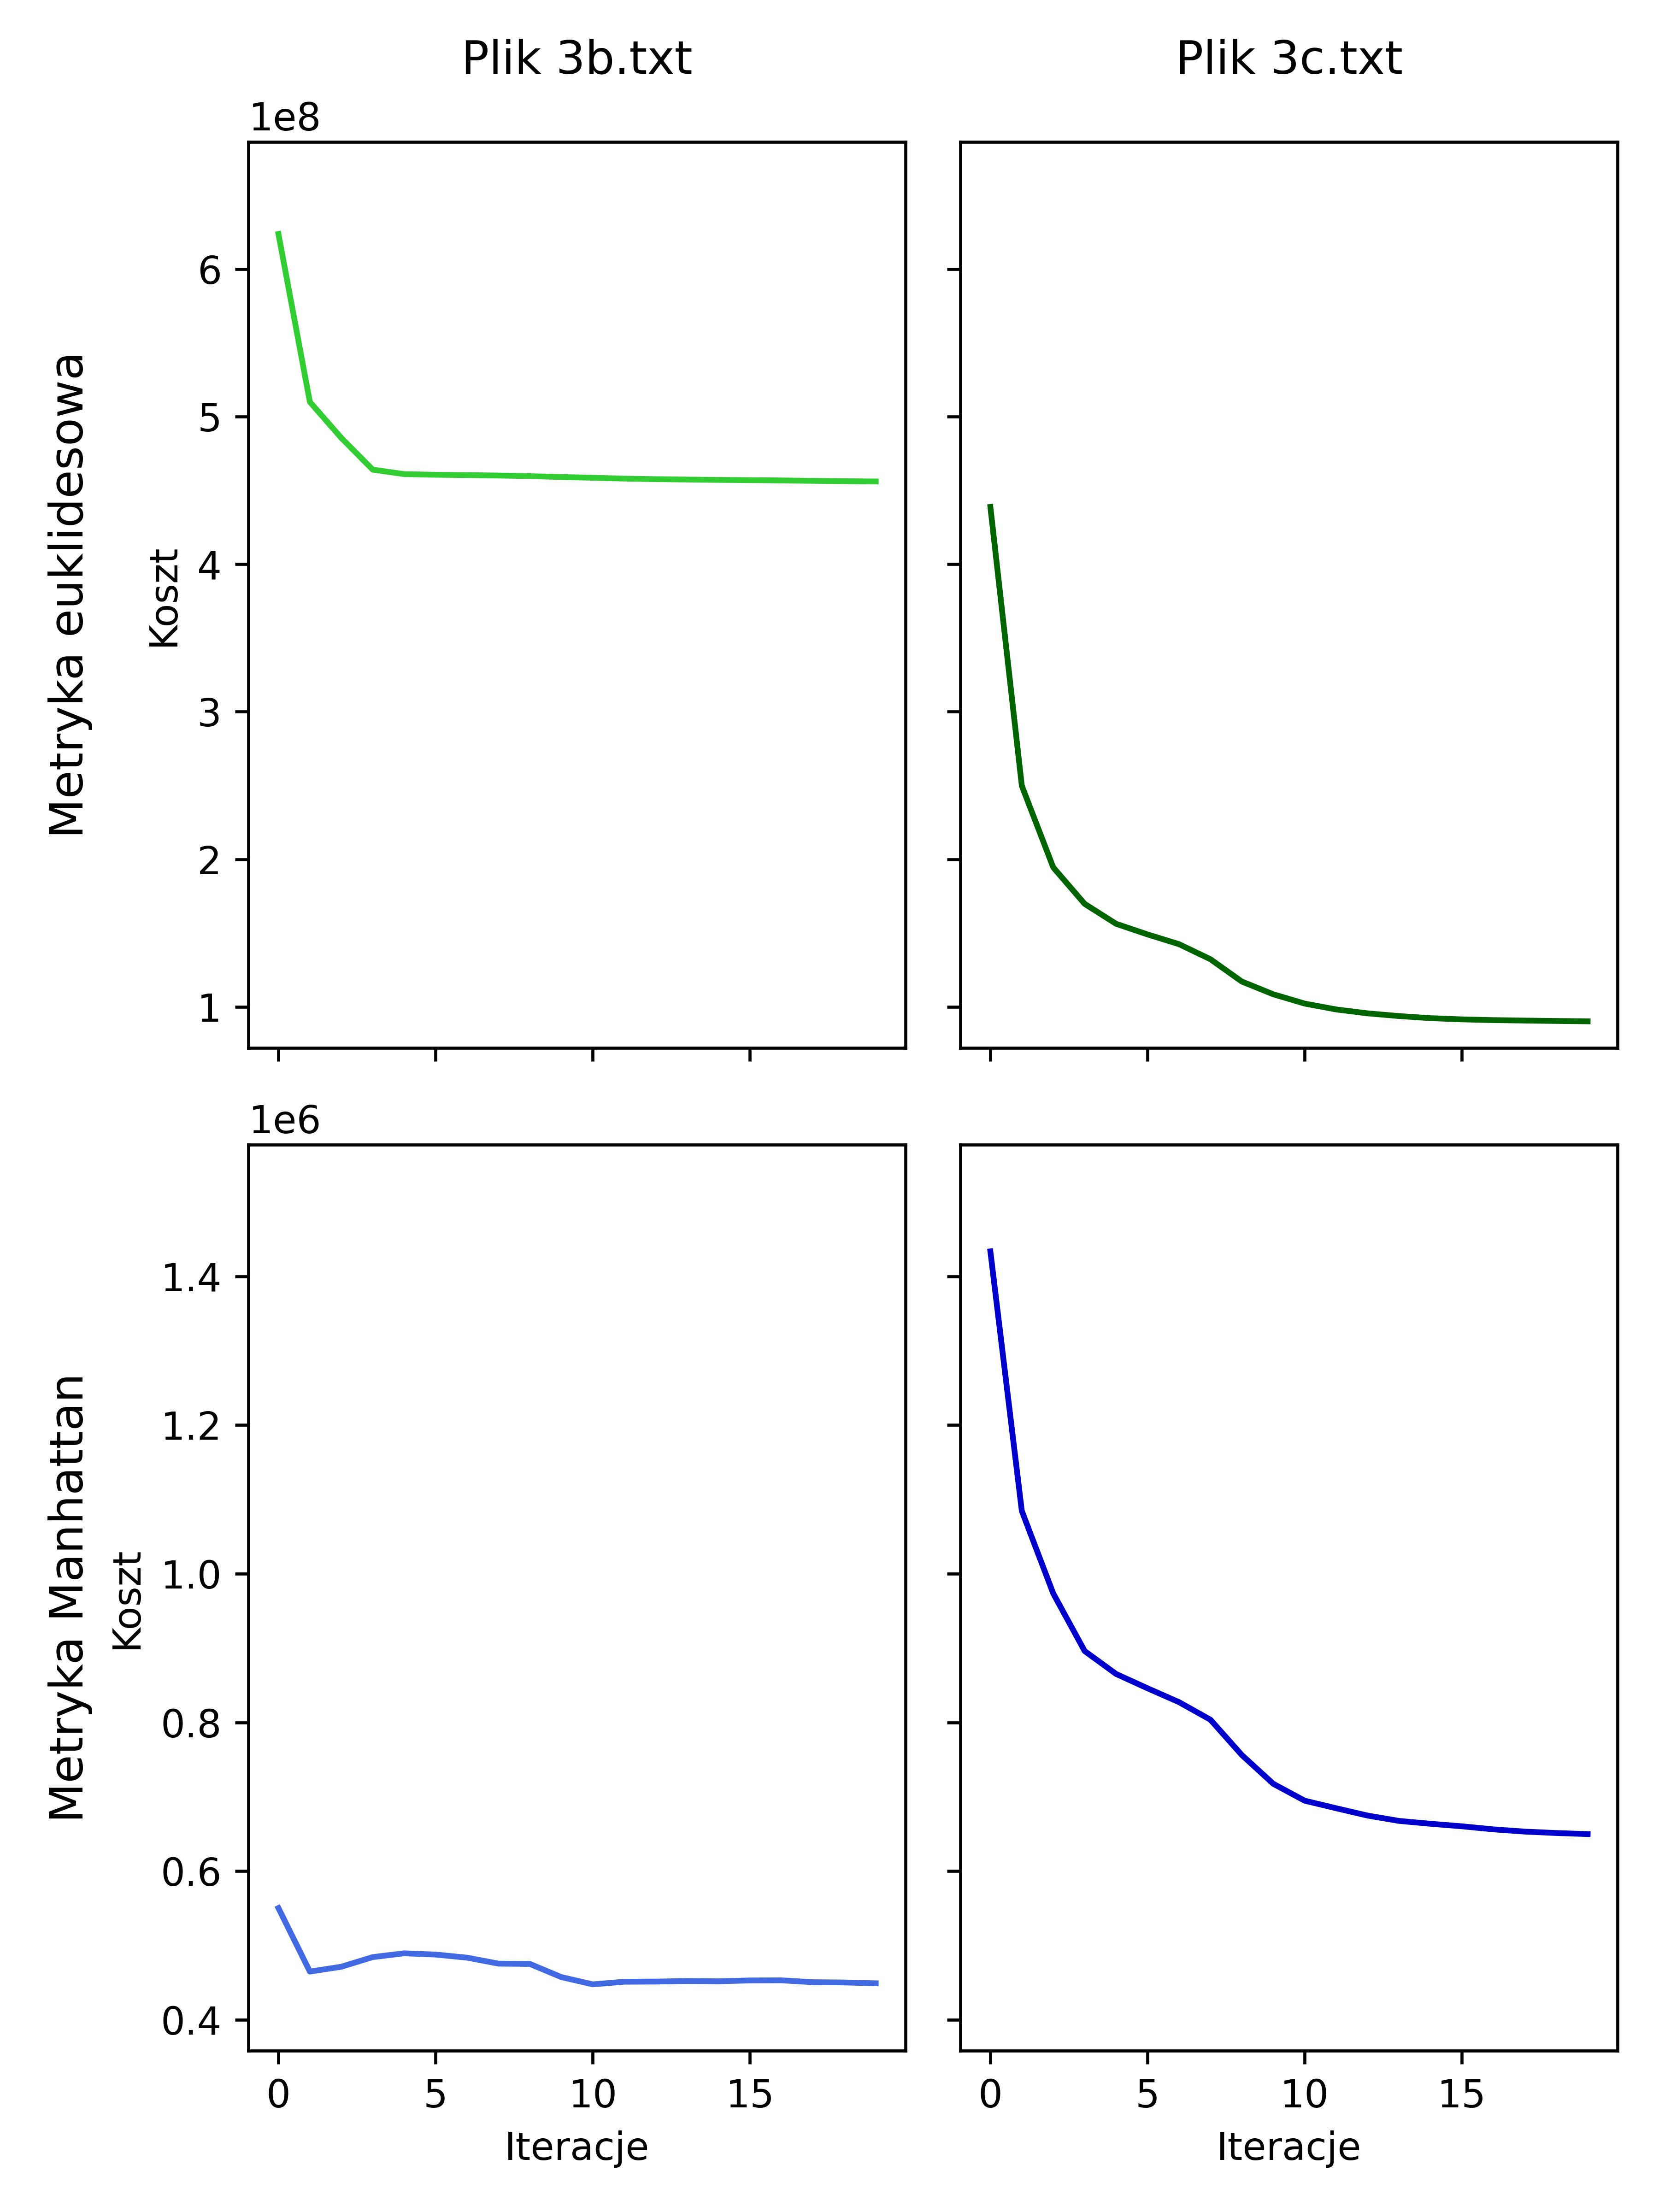
\includegraphics[width=1\textwidth]{img/zad3_fig.png}
    \caption{Wykresy funkcji kosztu}
	\end{center}
\end{figure}

\newpage
\section{Analiza wyników}

Wykresy funkcji (rysunek \ref{fig:chart}) celu dla identycznych początkowych skupień posiadają podobny kształt, co widać szczególnie dobrze w przypadku pliku \verb|3c.txt|, gdzie spadek kosztu robi się mniej gwałtowny po 4 iteracji, by delikatnie przyśpieszyć między 8 a 10 iteracją, po czym wykres zaczyna się widocznie wypłaszczać (co dokładniej można zobaczyć w tabeli \ref{tab:cost_results}).

W przypadku pliku \verb|3b.txt| kształt funkcji nie jest już tak zbliżony, głównie ze względu na fakt, że dla metryki Manhattan wartość funkcji celu nie zawsze maleje (wzrost można zaobserwować w iteracjach 3-5, 12-14 oraz 16-17). Niezależnie od metryki, kształt funkcji zaczyna się dużo wcześniej wypłaszczać niż w przypadku drugiego początkowego rozłożenia centroidów. 

Wniosek, że dla badanych początkowych środków skupień wykresy szybciej zaczynają się wypłaszczać w przypadku gdy centroidy są losowe (plik \verb|3b.txt|) widać także w tabeli \ref{tab:cost_change}. Zmiana kosztu jest prawie 3-krotnie większa dla maksymalnie oddalonych cenroidów. Wartości te są też większe dla metryki euklidesowej.

\end{document}
